%%------------------------------------------------------
%% Design for ECE Solutions Manual
%%------------------------------------------------------


% Excellent reference to the memoir package: https://www.ctan.org/pkg/memoir
\documentclass[letterpaper, 10pt]{memoir}
\chapterstyle{ger}
\settrims{0pt}{0pt}
\semiisopage[9]		% [N] is spine margin is 1/Nth pf page 

%%------------------------------------------------------
%% Document formatting standards.
%% references labels			figure:<camelCase>
%%						\tableofcontents:<camelCase>
%%						section:<dash seperated>
%%						index:<camelCase>
%%						example:<camelCase> 
%%						equ:<camelCase>
%%------------------------------------------------------

\usepackage{graphicx}
\usepackage{imakeidx}			% Enables Index functionality
\usepackage{hyperref}			% Enable hyperlinks to email and URLs

%% Lots of packages needed for tables
\usepackage{xcolor,colortbl}	% Enable colors in tables
\usepackage{multirow}
\usepackage{hhline}				% allows partial hlines in multirow tables
\usepackage{longtable}			%Enables multipage tables
\usepackage{makecell}			% deal with parboxes inside tables

\usepackage{amsmath}

\usepackage{tikz}			% Enable drawing simples shapes over text
\usepackage{subcaption}	% Enables tables to not have a caption but to increment the table counter


% Enables bars in the margin to follow example/solutions
\usepackage[color]{changebar}
\cbcolor{black}				
\setlength{\changebarwidth}{0.2cm}

\newcommand{\ul}{\underline}
\definecolor{Gray}{gray}{0.85}

\newcolumntype {g} {>{\columncolor{Gray}}c}



% Draws a item list bullet
\newcommand{\tabitem}{~~\llap{\textbullet}~~}


% I want all quotes to be in italics
\newenvironment{itquote}
{\begin{quote}\itshape}
{\end{quote}}

\newcounter{example}
\renewcommand{\theexample}{\thechapter.\arabic{example}}

\newenvironment{example}[1]% environment name
{% begin code
  \par\vspace{\baselineskip}\noindent
  \refstepcounter{example}%
  \cbstart%
  \textbf{Example \theexample} #1  %
  \par\vspace{\baselineskip}%
  \noindent\ignorespaces
}%
{% end code
  \cbend%
  \par\vspace{\baselineskip}%
  \noindent\ignorespacesafterend
}


%%		CHAPTER FORMATTING
%%  \chapter{The Engineering Design Process}
%% \label{chapter:engineeringDesignProcess}
%% \graphicspath{ {./chapter01/Fig} }
%% \begin{itquote}
%% \end{itquote}


%%		LONG TABLE FORMATTING



%%------------------------------------------------------
%%				Lessons Learned
%% If you want to use multirow with rowcolor:
%%		Color rows as usual
%%		Use multirow on the last row with negative row values
%%		You will need to use hhline for non-multirows
%%
%% Use 			\hphantom  \\		to insert a space between things
%%------------------------------------------------------




\begin{document}

\frontmatter
\title{{\Huge Design for Electrical and Computer Engineers} \\
				Theory, Concepts, and Practice\\
				Instructor's Solution Manual}
\author{Ralph M. Ford and Christopher S. Coulston}
\date{}
\maketitle


This document was prepared with \LaTeX.
\\
\\
\\

Copyright \copyright  2024 by Christopher Coulston
\\
\\

All rights reserved.  No part of this publication may be reproduced, 
stored in a retrieval system, or transmitted, in any form or by any
means, electronic, mechanical, photocopying, recording, or otherwise
without prior written permission of the author.


\tableofcontents


\mainmatter 					% Now Use Arabic numerals for page numbers

\textbf{Preface: How to Use This Manual}\\

This manual provides solutions to the problems found in 
\ul{Design for Electrical and Computer Engineers: Theory, Concepts, and Practice}. 
For guidance to instructor’s we identify problems as
either: review, application, and project. Review-type problems usually ask the student to restate
an important concept from the text, whereas application problems are those where the students
are required to solve a more in-depth project that demonstrates an understanding of the concepts
learned to a new scenario. Project problems are important steps in the completion of a senior
capstone design project. Each particular problem is categorized in this solutions manual as to the
type of problem it is by using the key [R], [A], and [P].\\

Furthermore, we also provide our guidance (identified in the manual as Notes), from experience
teaching the material, with pointers on how we present the material and apply it to student
projects. Selected project assignments are also supplied.\\


\textit{We also ask that instructor’s keep this manual for instructor use only and do not post or
otherwise distribute our solutions in any form. Unfortunately, it is becoming all too common
for solutions to be copied and distributed over the Internet, thus hurting other instructors
using the book.}

\textbf{Feedback}\\
Feedback and suggestions concerning any aspect of this manual, that would likely benefit the
overall presentation, would be much appreciated. Please send your comments via email to
Ralph-Ford@psu.edu or coulston@mines.edu

\showanswers
\chapter{The Engineering Design Process}
\section{Problems}
\label{problems}

\begin{enumerate}
\itemsep0em 
\def\labelenumi{\arabic{enumi}.}
\item
  In your own words, describe the difference between prescriptive and
  descriptive design processes. Cite examples of each.
\item
  Describe the relationship between the Problem Identification,
  Research, and Requirements Specification phases of the design process.
\item
  Describe the relationship between the Concept Generation and Design
  phases of the design process.
\item
  Construct a prescriptive design process for the Problem
  Identification, Research, Specification, Concept, and Design phases of
  the design process. The result should be a flow chart that contains
  decision blocks and iteration as necessary.
\item
  Describe the main differences between the VLSI and embedded system
  design processes.
\item
  Using the library or Internet, conduct research on the spiral software
  design process.

\begin{enumerate}
\itemsep0em 
\def\labelenumi{\alph{enumi})}
\item
  Outline the significant elements of the spiral software design
  process.
\item
  Describe the advantages and disadvantages of this relative to the
  waterfall model?
\end{enumerate}

\begin{quote}
Cite all reference used.
\end{quote}

\item
  Using the library or Internet, conduct research on the Extreme
  Programming design process.

\begin{enumerate}
\itemsep0em 
\def\labelenumi{\alph{enumi})}
\item
  Outline the significant elements of the Extreme Programming paradigm.
\item
  What are the pro and con arguments for this software development
  model?
\end{enumerate}

\begin{quote}
Be sure to cite references.
\end{quote}

\item
  \textbf{Project Application.} In preparation for project and team
  selection, develop a personal inventory that includes a list of five
  favorite technologies or engineering subjects that you are interested
  in pursuing. Also, list the strengths and weaknesses that you bring to
  a project team.
\end{enumerate}


\chapter{Project Selection and Needs Identification}
\section{Problems}
\label{section:problems}


\begin{enumerate}
\def\labelenumi{\arabic{enumi}.}
\item
  In your own words, describe the differences between creative, variant,
  and routine designs.
 \begin{onlysolution}
 \textbf{[R]}
 \itshape
 Creative designs are typically new and innovative design ideas -- those
that did not exist before. Variant designs are variations of existing
designs, with the intent of improving some aspect of the existing
system. Routine designs are concerned with fairly well-known artifacts
for which there is a well-developed design knowledge base.
  \end{onlysolution}
  
\item
  List three guidelines that should be employed when selecting a
  project.
\item
  Assume a customer comes to you with the following
  request---\emph{Design a mechanical arm to pick apples from a tree}.
  What are the assumptions in this statement? Rewrite the request to
  eliminate the assumptions. (This problem was originally posed by
  Edward DeBono {[}Deb70{]}).
\item
  Assume a customer comes to you with the following
  request---\emph{Design an RS-232 networked personal computer
  measurement system to transmit voltage measurements from a remote
  location to a central server.} What are the assumptions this
  statement? Develop a list of questions that you might ask the customer
  to further clarify the problem statement.
\item
  Describe what is meant by a marketing requirement.
\item
  What is the purpose of an objective tree and how is it developed?
\item
  The needs for a garage door opener have been determined to be: safety,
  speed, security, reliability, and noise. Create a pairwise comparison
  to determine the relative weights of the needs. Apply your judgment in
  making the relative comparisons.
\item
  Consider the design of an everyday consumer device such as computer
  printer, digital camera, electric screwdriver, or electric toothbrush.
  Determine the customer needs for the device selected. The deliverables
  should be: 1) marketing requirements, 2) an objective tree, and 3) a
  ranking of the customer needs using pairwise comparison.
\item
  \textbf{Project Application.} Select criteria to be applied for
  selecting a project concept as shown in Example~\ref{example:projectSelectionModel}
  then brainstorm and search to generate project concepts. Rank the top three to five
  concepts against the criteria as presented in Example~\ref{example:projectSelectionModel}.
\item
  \textbf{Project Application.} Determine the needs for the project
  selected. The result should be list of marketing requirements, an
  objective tree, and a ranking of the needs.
\item
  \textbf{Project Application.} Conduct a research survey for your
  project using the guidance presented in Section~\ref{section:needs-identification}. The result should
  be a report summarizing the results of the survey.
\item
  \textbf{Project Application.} Develop a Problem Statement for your
  project concept as outlined in Section~\ref{section:project-application-the-problem-statement}. 
  Apply the processes
  presented in the chapter as appropriate.
\end{enumerate}


\chapter{The Requirements Specification}
\section{Problems}
\label{section:reqSpecProblems}
\graphicspath{ {./chapter03/FigSolutions} }

\begin{enumerate}
\def\labelenumi{\arabic{enumi}.}
\item
  Briefly describe the four properties of an engineering requirement.
  
  
\item
  Identify the three levels of standards usage and what is meant by each one.
  
 \begin{onlysolution}
 \textbf{[R]}
 \itshape
  The three levels of standards usage are user, implementation, and
development. The \textbf{user level} simply incorporates the standard
within the design without the need for technical knowledge concerning
the standard. However, the \textbf{implementation level} requires an
in-depth knowledge of the standard -- developing hardware drivers and
ensuring reliability requirements. As with the implementation level, the
\textbf{development level} also requires knowledge of the standard in
order to further develop and modify its predecessor.
\end{onlysolution}
  
  
\item
  For each of the engineering requirements below, determine if it meets
  the properties of abstractness, unambiguous, verifiable, and
  realistic. If a requirement does not satisfy the properties, restate
  it so that it does:


\begin{enumerate}
\def\labelenumi{\alph{enumi})}
\item
  The TV remote control will be easy to use.
  
\begin{onlysolution}
\textbf{[A]}
 \itshape
 Abstractness: \textbf{Yes} -- doesn't give details on implementation\\
Unambiguous: \textbf{Maybe} -- there is not a clear definition of
easy-to-use. It could be possible to develop some metrics for easy to
use, such as size of buttons, number of buttons, etc.\\
Verifiable: \textbf{Maybe -} this relates back to the ambiguity of
easy-to-use. If the easy-to-use property is defined, then it could be
verifiable.
\end{onlysolution}
  
  
\item
  The robot will identify objects in its path using ultrasonic sensors.
  
\begin{onlysolution}
\textbf{[A]}
 \itshape
Abstractness: \textbf{No} -- provides a solution to the problem (ultrasonic sensors)\\
Unambiguous: \textbf{No} -- it will identify objects in its path, is
somewhat clear. However, could be better defined if its path were
defined, as well as the distance of detection\\
Verifiable: \textbf{No} (Because it is not unambiguous.)\\
\textbf{Restatement:} ``The robot will identify objects in its forward
path within 3 feet of the robot.''
\end{onlysolution}

\item
  The car audio amplifier will be encased in aluminum and will operate
  in the automobile environment.
  
  \begin{onlysolution}
  \textbf{[A]}
   \itshape
Abstractness: \textbf{No} -- provides a solution to the problem (aluminum case)\\
Unambiguous: \textbf{No} -- it will operate in an automobile is not
quite clear. Where in the automobile and what size should it be?\\
Verifiable: \textbf{No --} because it is not unambiguous.\\
\textbf{Restatement:} ``The car audio amplifier will operate in the
automobile passgenger compartment and not have a size that exceeds
12''x4''6'' ''
\end{onlysolution}

\item
  The audio amplifier will have a total harmonic distortion that is less
  than 2\%.
  
  \begin{onlysolution}
  \textbf{[A]}
   \itshape
Abstractness: \textbf{Yes} -- doesn't give details on implementation \\
Unambiguous: \textbf{Yes} -- THD \textless{} 2\%  \\
Verifiable: \textbf{Yes}
\end{onlysolution}

\item
  The robot will be able to move at speed of 1 foot/sec in any
  direction.
  
  \begin{onlysolution}
  \textbf{[A]}
   \itshape
Abstractness: \textbf{Yes} -- doesn't give details on implementation \\
Unambiguous: \textbf{No} -- provides two requirements in one statement \\
Verifiable: \textbf{Yes} \\
\textbf{Restatement:} ``The robot will be able to move at a speed of 1 foot/sec.'' or
``The robot will be able to move in any direction.''
\end{onlysolution}

\item
  The system will employ smart power monitoring technology to achieve
  ultra-low power consumption.
  
  \begin{onlysolution}
  \textbf{[A]}
   \itshape
Abstractness: \textbf{No} -- provides a solution to the problem (smart power)\\
Unambiguous: \textbf{Yes} -- it will achieve ultra-low power consumption \\
Verifiable: \textbf{No} -- there is no exact target value on the power \\
\textbf{Restatement:} ``The system will achieve power consumption below XX watts.''
\end{onlysolution}

\item
  The system shall be easy to use by a 12 year old.
  
  \begin{onlysolution}
  \textbf{[A]}
   \itshape
Abstractness: \textbf{Yes} -- doesn't give details on implementation\\
Unambiguous: \textbf{Maybe} -- a 12 year old can use this device is
clear, but as we saw in an earlier problem it is hard to determine ease
of use without some sort of definition.\\
Verifiable: \textbf{Yes}\\
\end{onlysolution}

\item
  The robot must remain operational for 50 years.
  
  \begin{onlysolution}
  \textbf{[A]}
   \itshape
Abstractness: \textbf{Yes} -- doesn't give details on implementation\\
Unambiguous: \textbf{No} -- Failure is a probability-based concept.  A single 
robot always a non-zero chance of failure over an extended periodn of time.\\
Verifiable: \textbf{No} - As a practical matter, your design team would not be
able to perform this test.\\
\end{onlysolution}

\end{enumerate}

  \item
    Provide three example engineering requirements that are technically
    verifiable, but not realistic.
    
  \item
    Describe the difference between \emph{verification} and  \emph{validation}.
    
\begin{onlysolution}
 \textbf{[R]}
 \itshape
Validation is the process of determining if the requirements meet the
needs of the end-user. This answer the question -- are we building the
right product? Verification is the process of measuring or demonstrating
that the requirements are met in the final realization. Verification
answers the question -- are we building the product right (does it meet
the requirements).

Validation is typically harder to determine.
\end{onlysolution}    
    
    
    
    
  \item
    Explain how \emph{validation} is performed for a Requirements Specification.
    
\begin{onlysolution}
  \textbf{[R]}
   \itshape
Validation can be performed by being able to answer the following
questions affirmatively:

\begin{itemize}
\item \textbf{Is each requirement verifiable?} That is can it be measured or
shown in the final system implementation.
\item \textbf{Is each requirement traceable to a user requirement?}
\item \textbf{Is each requirement realistic and technically feasible?} This
may be hard to determine. It can be determined based upon benchmarks or
system prototypes.
\item \textbf{Is the property of orthogonality met for the Requirements
Specification?} Are the requirements established with no redundancy?
\item \textbf{Is the property of completeness met?} Are all the needs of the
end-user addressed in the Requirements Specification?
\item \textbf{Is the property of consistency met?} The Requirements
Specification should not be self-contradictory.
\end{itemize}
\end{onlysolution}    
    
  \item
    Provide an example of a project (real or fictitious) where
    verification is successful, but validation is unsuccessful.
    
%Question 3.8 Use PDF 3.6    
  \item
  \label{list:identifyMarkEngr}
    Consider the design of a common device such as an audio CD player,
    an electric toothbrush, or a laptop computer (or another device that
    you select). Identify potential marketing and engineering
    requirements. Consider those categories presented in 
    Section~\ref{section:engineering-requirements}, as
    well as any others that are applicable to the problem. You do not
    need to select the target values, but should identify the measures
    and units. Present the requirements in a table format as in 
    Table~\ref{table:audioRequireSpec}.
    
 \begin{onlysolution}
   \textbf{[A]}
   \itshape
 \textbf{Marketing Requirements}
\begin{itemize}
\item Should be lightweight
\item Clean teeth well.
\item Have a long battery life.
\item Not shock the user (electric).
\item Be easy to hold
\item Be quiet.
\item Easy to clean.
\item Be lightweight.
\item Allow multiple users.
\end{itemize} 

\begin{tabular}{m{6cm}|m{6cm}}
Engineering Requirements & Notes \\ \hline

%\multicolumn{2}{l}{Performance} \\ \hline

E1.Have \_\_\_ ft-lbs of torque (or translational force, depending upon design). &
This addresses how much force it can apply in cleaning the teeth. This
requirement does require assuming part of the solution.	\\ \hline

E2.Should have a rotational/translational brush speed of \_\_\_
cycles/minute (Note some of the solution assumed here). &
This addresses how quickly it the toothbrush operated.				\\ \hline

E3.Must have a reliability of 95\% at 5 years of service. &
Reliability -- may be a good idea to place an estimate on this. This is
a real guess, and one would have to do more work to determine this one.	\\ \hline

E4. Should emit \textless{} \_\_\_ dB of noise. &
User wanted it to be quiet						 \\ \hline

%\multicolumn{2}{l}{Environmental} \\ \hline

E5. Must work in 100\% humidity (could be submersed). &
Works in a wet environment. Could be submersed.		 \\ \hline

E6.Must be able to withstand \_\_\_ drop from 6 feet and still operate
motor (not brush head). &
User could drop it. 6 feet is typical person height.		\\ \hline

E7.Temperature range of \_\_\_ to \_\_\_\_ degrees Celsius.		\\ \hline

%\multicolumn{2}{l}{Energy} \\ \hline

E8.Should have an operating lifetime of \textgreater{} \_\_\_ hours on a
single battery (or charge). &
How long it will run for.			\\ \hline

%\multicolumn{2}{l}{Packaging/Physical Characteristics} \\ \hline
E9.Toothbrush should weigh less than \_\_ grams. &
Do not want it to be too heavy.			\\ \hline

E10. Should be \_\_\_ cm tall. &
Height should be specified. Should not be too long nor too short.			\\ \hline

%\multicolumn{2}{l}{Cost} \\ \hline

E11. Should cost no more than \$\_\_\_ to produce. &
Cost is virtually always an issue.			\\ \hline
\end{tabular}

 \end{onlysolution}    
    
    
    
    
%Question 3.9 Use PDF 3.7    
  \item
    Develop a marketing-engineering tradeoff matrix for the device
    selected in Problem~\ref{list:identifyMarkEngr}.
    

    
 \begin{onlysolution}
   \textbf{[A]}
   \itshape

\begin{tabular}{l|l|l|l|l|l|l|l|l|l|l|l|l|} 
\multicolumn{2}{l|}{} & 
		 		\rotatebox[origin=c]{90}{E1. Torque} &
  				\rotatebox[origin=c]{90}{E2. Brush Speed}  &
  				\rotatebox[origin=c]{90}{E3. Reliability}  &
  				\rotatebox[origin=c]{90}{E4. Noise}  &
  				\rotatebox[origin=c]{90}{E5. Humidity}  &
  				\rotatebox[origin=c]{90}{E6. Shock Res.}  &
  				\rotatebox[origin=c]{90}{E7. Temp. }  &
  				\rotatebox[origin=c]{90}{E8. Battery Life }  &
  				\rotatebox[origin=c]{90}{E9. Weight }  &
  				\rotatebox[origin=c]{90}{E10. Size }  &
  				\rotatebox[origin=c]{90}{E11. Cost }  \\ \hline
  				
\multicolumn{2}{l|}{}              &  +   & + & +   &  -   & + & +  & + & + & - & -  & -     \\ \hline
M1. Lightweight 		& - &     $\downarrow$ & 	&     $\downarrow$ &    $\downarrow$  & &     $\uparrow$ & & $\downarrow$ &$\uparrow$   & $\uparrow$  &      $\downarrow$ \\ \hline
M2. Cleans Well		& + &     &   $\uparrow$ &     &     & &   & & & $\downarrow$  & $\downarrow$ &    \\ \hline
M3. Long Life		& +&     & 	$\downarrow$ & $\downarrow$     &     & &  $\uparrow$  &$\uparrow$  & $\uparrow$ & $\downarrow$  & &    \\ \hline
M4. Electric shock		& + &     & 	&     &     &  $\uparrow$ &   & & &  & &    \\ \hline
M5. Easy to hold		& + &  $\downarrow$   & 	&     &     & & $\downarrow$  & & $\downarrow$ & $\uparrow$ &$\uparrow$ &  $\downarrow$  \\ \hline
M6. Quiet			& +&  $\downarrow$     &  $\downarrow$ 	&     & $\uparrow$     & &   & & &  &  $\downarrow$  &  $\downarrow$    \\ \hline
M7. Durable		& + &     & 	& $\uparrow$     &     &$\uparrow$  & $\uparrow$   &$\uparrow$  & &  & &  $\downarrow$   \\ \hline
\end{tabular}

 \end{onlysolution}
    
 %Question 3.10 Use PDF 3.8
  \item
    Develop an engineering tradeoff matrix for the device selected in
    Problem~\ref{list:identifyMarkEngr}.
    
 \begin{onlysolution}
    \textbf{[A]}
   \itshape

\begin{tabular}{l|l|l|l|l|l|l|l|l|l|l|l|l|} 
\multicolumn{2}{l|}{} & 
				\rotatebox[origin=c]{90}{E1. Torque} &
  				\rotatebox[origin=c]{90}{E2. Brush Speed}  &
  				\rotatebox[origin=c]{90}{E3. Reliability}  &
  				\rotatebox[origin=c]{90}{E4. Noise Level}  &
  				\rotatebox[origin=c]{90}{E5. Humidity}  &
  				\rotatebox[origin=c]{90}{E6. Phys. Shock }  &
  				\rotatebox[origin=c]{90}{E7. Temp. }  &
  				\rotatebox[origin=c]{90}{E8. Battery Life }  &
  				\rotatebox[origin=c]{90}{E9. Weight }  &
  				\rotatebox[origin=c]{90}{E10. Size }  &
  				\rotatebox[origin=c]{90}{E11. Cost }  \\ \hline
\multicolumn{2}{l|}{}       &  +   & + & +   &  -   & + & +  & + & + & - & -  & -     \\ \hline  				
E1. Torque 		& + &  \cellcolor{lightgray}&  $\downarrow$  & & & & & &  $\downarrow$ & $\downarrow$  & $\downarrow$  &  $\downarrow$  \\ \hline
E2. Brush Speed	& + &\cellcolor{lightgray} & \cellcolor{lightgray}& &$\downarrow$  & & & & $\downarrow$ &  && $\downarrow$\\ \hline
E3.  Reliability	& +&   \cellcolor{lightgray}& \cellcolor{lightgray}& \cellcolor{lightgray}& & $\uparrow$& $\uparrow$& $\uparrow$& & $\downarrow$ &$\downarrow$ &$\downarrow$\\ \hline
E4. Noise Level	& - &  \cellcolor{lightgray}  & \cellcolor{lightgray}& \cellcolor{lightgray}& \cellcolor{lightgray}& & & & & $\downarrow$ & $\downarrow$&$\downarrow$ \\ \hline
E5. Humidity	& + &  \cellcolor{lightgray}& \cellcolor{lightgray}&\cellcolor{lightgray} & \cellcolor{lightgray}& \cellcolor{lightgray}& & & & $\downarrow$ &   & \\ \hline
E6. Phys. Shock	& +&  \cellcolor{lightgray}& \cellcolor{lightgray}&\cellcolor{lightgray} &\cellcolor{lightgray} &\cellcolor{lightgray} & \cellcolor{lightgray}& & & $\downarrow$ & $\downarrow$  & \\ \hline
E7. Temerature	& + & \cellcolor{lightgray}  & \cellcolor{lightgray}&\cellcolor{lightgray} & \cellcolor{lightgray}& \cellcolor{lightgray}& \cellcolor{lightgray}& \cellcolor{lightgray}& \cellcolor{lightgray}& &   & $\downarrow$\\ \hline
E8. Battery Life	& + &  \cellcolor{lightgray} & \cellcolor{lightgray}&\cellcolor{lightgray} &\cellcolor{lightgray} & \cellcolor{lightgray}& \cellcolor{lightgray}&\cellcolor{lightgray} & \cellcolor{lightgray}& $\downarrow$&  $\downarrow$ & $\downarrow$\\ \hline
E9. Weight		& - &   \cellcolor{lightgray} &\cellcolor{lightgray}&\cellcolor{lightgray}& \cellcolor{lightgray}& \cellcolor{lightgray}& \cellcolor{lightgray}& \cellcolor{lightgray}& \cellcolor{lightgray}&  \cellcolor{lightgray}& $\downarrow$  & $\downarrow$\\ \hline
\end{tabular}
 \end{onlysolution}

 %Question 3.11 Use PDF 3.11
  \item
    Develop a list of potential standards that would apply to one of the
    devices proposed in Problem~\ref{list:identifyMarkEngr}, and for each indicate how it would
    apply to the design.
    
\begin{onlysolution}
    \textbf{[A]}
   \itshape
\textbf{Standards for the Electric Toothbrush}
Likely standards for this system include:\\
UL (Underwriters Laboratory) and CE (Common European) safety standards.
This is very common for consumer devices.\\
ADA -- American Dental Association. This would likely be a series of
``standard'' tests before branding ADA approval; therefore, showing that
this system provides sufficient dental treatment.
\end{onlysolution}    

    
  \item
    \textbf{Project Application.} Develop a complete requirements
    document for your project as outlined in 
    Section~\ref{section:project-application-the-requirements-specification}. Make sure that
    the engineering requirements meet the five properties identified in
    the chapter. The team should complete the self-assessment checklist
    in Table~\ref{table:requirementsCheckList}.
    
    
\begin{onlysolution}
    \textbf{[P]}
   \itshape    
   
\textbf{Note:} The \textul{Requirements Specification} is an
important document in the design. Remember that requirement specifications are ``living'' and evolving
documents. Thus it is a good idea to provide design teams with the opportunity to resubmit and
revise the document. We use a two-step submission process. The first submission is
worth 30\% of the specification grade. This is reviewed and resubmitted to the team,
who resubmits, and the second submission constitutes the remaining 70\%. Of course,
if the team gets it right on the first submission, there is no need to resubmit.

\textbf{Constraints}. We have student teams identify at least
five of eight constraints in their specification. They should be
realistic. We don't require that they test each one in the final

realization, but ensure that they are considered (this depends upon the
complexity of the problem). However, the team should be able to that
their system would meet some of the constraints.

Students may also make the counter argument for a constraint. For
example, design team may consider a constraint category, and determine
that it is not applicable. If a clear rationale is given, the team could
document that. If a project has virtually no constraints, then must
question whether or not it is an acceptable project.

\textbf{Standards}. We have students identify standards that
may apply to their project. Of course, they may not know all of
the applicable standards until they get to the design phase.
However, realistic decisions can be made on the standards that will
apply to the project. Some of them may be very beneficial to the design
team. For example, following design standards, such as the IEEE software
design standards can be of great help to the teams.

\textbf{Checklist.} We expect our student teams to also complete
the self-assessment checklist for requirements provided in Table 3.7.

\textbf{Oral Presentations.} After the students complete the
Requirements Specification, we have them make a presentation to a
faculty group. This presentation covers the Problem Statement material
from Chapter 2, the Requirements, Constraints, and Standards. The idea
is for the faculty to make accept/reject the project idea, or more
likely, request changes/corrections.

We also pick one or two teams to present theirs to the entire class
prior to the faculty presentations. This way students can
critique a presentation before hand.

\end{onlysolution}

\end{enumerate}

\chapter{Concept Generation and Evaluation}
\section{Problems}
\label{section:problems}

\begin{enumerate}
\def\labelenumi{\arabic{enumi}.}
\item
  Consider the nine dot puzzle shown in Figure 4.1 (b). Draw
  \textbf{three} connected straight lines that pass through all nine
  dots.

\item
  Consider the six sticks shown below. Rearrange the sticks to produce
  four equilat­eral triangles (the sticks cannot be broken).
\item
  Consider the fish shown below made of eight sticks and a coin for the
  eye. The objective is to make the fish face the other direction by
  moving only the coin and three sticks.

\begin{figure}
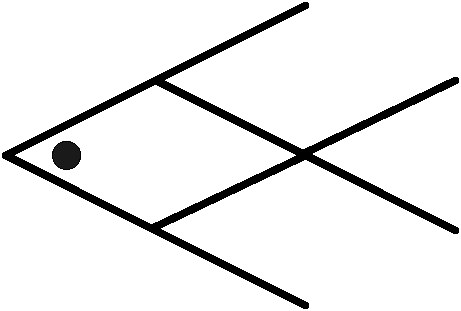
\includegraphics[width=2in,height=1.35in]{image34.pdf}
\label{figure:dotsProblems}
\end{figure}

\item
  For each of the following lateral thinking puzzles, develop a
  plausible solution (from Paul Sloane's \ul{Lateral Thinking Puzzles}
  {[}http://dspace.dial.pipex.com/sloane{]}):

\begin{itemize}
\item
  A man walks into a bar and asks the barman for a glass of water. The
  barman pulls out a gun and points it at the man. The man says
  \textquotesingle Thank you\textquotesingle{} and walks out.
\item
  A woman had two sons who were born on the same hour of the same day of
  the same year. But they were not twins. How could this be so?
\item
  Why is it better to have round manhole covers than square ones?
\item
  A man went to a party and drank some of the punch. He then left early.
  Everyone else at the party who drank the punch subsequently died of
  poisoning. Why did the man not die?
\end{itemize}

\item
  Legislation was passed to allow handguns in the cockpits of passenger
  airliners to prevent hijacking. Brainstorm to develop concepts that
  prevent anyone other than the pilot from using the handgun.
\item
  Imagine if scientists and engineers were able to develop a technology
  that would allow people to be transported from any place on earth to
  another instantaneously. Brainstorm to determine the potential impact
  this would have on society.
\item
  Student advising at many colleges and universities is seen as an area
  that can be im­proved. Brainstorm to develop ideas as to how student
  advising could be improved at your college or university.
\item
  In your own words, describe what a concept table and a concept fan
  are.
\item
  Consider the problem solved in Section 4.3.2. For this example assume
  that:
\begin{itemize}

\item
  The following is the result of the paired comparison.

\begin{table}
\begin{tabular}{|c|c|c|c|c|}
\hline
              &
Accuracy &
Cost &
Size &
Availability \\ \hline
Accuracy & 1 & 1/3 & 2 & ½ \\ \hline
Cost & 3 & 1 & 5 & 1 \\ \hline
Size & 1/2 & 1/5 & 1 & 2 \\ \hline
Availability & 2 & 1 & ½ & 1 \\ \hline
\end{tabular}
\end{table}


\item
  The parts costs are the following: resistors = \$0.05, bipolar
  transistors (BJTs) = \$0.10, op amps = \$0.35, and RTDs = \$0.25.
\item
  The parts have an in-stock availability of 99\%, 90\%, 85\%, and 70\%
  of the time for the re­sistors, BJTs, RTDs, and op amps respectively.
\item
  Everything else is the same as presented in Section 4.3.2.
\end{itemize}

Compute the rankings of the design options using a weighted decision
matrix of the type shown in Table 4.5.


\item
  \textbf{Project Application.} Utilize the methods in this chapter to
  generate con­cepts for your particular design problem. Critically
  evaluate the concepts generated using one or more of the techniques
  presented in the chapter that is appropriate for the problem. Section
  4.4 pro­vides guidance on how to conduct this process and document the
  results.
\end{enumerate}



\begin{comment}
\section{Problems}
\label{section:problems}

\begin{enumerate}
\def\labelenumi{\arabic{enumi}.}
\item
  Describe the differences between \emph{bottom-up} and \emph{top-down}
  design.
\item
  Develop a functional design for an audio graphic equalizer. A graphic
  equalizer decomposes an audio signal into component frequencies bands,
  allows the user to apply amplification to each individual band, and
  recombines the component signals. The design can employ either analog
  or digital processing. Be sure to clearly identify the design levels,
  functional requirements, and theory of operation for the different
  levels in the architecture.

The system must
\begin{itemize}
\item
  Accept an audio input signal source, with a source resistance of 1000Ω
  and a maximum input voltage of 1V peak-to-peak.
\item
  Have an adjustable volume control.
\item
  Deliver a maximum of 40W to an 8Ω speaker.
\item
  Have four frequency bands into which the audio is decomposed (you
  select the frequency ranges).
\item
  Operate from standard wall outlet power, 120V rms.
  \end{itemize}
  
  \item
    Develop a functional design for a system that measures and displays
    the speed of a bicycle. Be sure to clearly identify the design
    levels, functional requirements, and theory of operation for each
    level.\\
  The system must

\begin{itemize}
\item
  Measure instantaneous velocities between zero and 75 miles per hour
  with an accuracy of 1\% of full scale.
\item
  Display the velocity digitally and include one digit beyond the
  decimal point.
\item
  Operate with bicycle tires that have 19, 24, 26, and 27 inch
  diameters.
\end{itemize}

  \item
    Draw a structure chart for the following C++ program:
\begin{verbatim}
void IncBy5(int \&a, int \&b);
int Multiply(int a, int b);
void Print(int a, int b);

main() {
    int x=y=z=0;
    IncBy5(x,y);
    z=Mult(x,y);
    Print(x,z);
}

void IncBy5(int \&a, int \&b) {
    a+=5;
    b+=5;
    Print(a,b);
}

int Multiply(int a, int b) {
    return (a*b);
}

void Print(int a, int b) {
    cout  << a << ``, `` << b;
}
\end{verbatim}

\item
  Develop a functional design for software that meets the following
  requirements. \\
The system must

\begin{itemize}
\item
  Read an array of floating point numbers from an ASCII file on disk.
\item
  Compute the average, median, and standard deviation of the numbers.
\item
  Store the average, median, and standard deviation values on disk.
\end{itemize}

The design should have multiple modules and include the following
elements: (a) a structure chart, and (b) a functional description of
each module.



\item
  Describe in your own words what is meant by coupling in design.
  Describe the advantages of both loosely and tightly coupled designs.
\item
  \textbf{Project Application.} Develop a functional design for your
  project. Follow the presentation guidelines in Section 5.9 for
  communicating the results of the design.
\end{enumerate}


\section{Problems}
\label{section:behavModelsProblems}

\begin{enumerate}
\def\labelenumi{\arabic{enumi}.}
\item
  Why is it important for a model to separate the design of a system
  from its realization?

\item
  Classify each of the following as either a model, not a model, or
  sometimes a model. Justify your answer based on the definition and
  properties of a model.

\begin{itemize}
\def\labelenumi{\alph{enumi})}
\item A diagram of a subway system,
\item a computer program, 
\item a football play, 
\item drivers license,
\item a floor plan of the local shopping mall (a ``you are here'' diagram)., 
\item an equation, 
\item A scratch n' sniff perfume advertisement in a fashion magazine,
\item The 1812 overture,
\item a braille sign reading ``second floor'',
\item sheet music for the Brandenburg Concerto, 
\item the United States Constitution, 
\item a set of car keys,
\item the ASCII encoding of an email message.
\end{itemize}


  \item
    Which of the following systems has memory? Justify your answer using
    the concepts of input, output, and state.
\begin{itemize}
\def\labelenumi{\alph{enumi})}
\item  an ink pen,
\item a resistor,
\item a capacitor,
\item a motorized garage door,
 \item an analog wrist watch, 
\item the air pressure in an air compressor, 
\item  the thermostat which controls the furnace in a house, 
\item a light switch, 
\item a political system,
\item the temperature of a large lake, 
\item  a book, 
\item a computer's hard drive.
\end{itemize}


  \item
    A can of soda has memory. Your objective is to figure out what
    characteristic of the can is the state variable and what input
    causes it to change. Based upon this, draw a state diagram for a can
    of soda. Label the transition arcs with the input responsible for
    the transition. Hint: no special equipment is needed to elicit the
    change of state.
  \item
    Consider the state diagram for the vending machine shown in 
    Table~\ref{table:stateVendingMachine}.
    Now assume that the system accepts nickels, dimes, and
    quarters. Also assume that it is capable of returning change to the
    user after a purchase. Create a state diagram that represents this
    new system. Make sure to define the output signals and their value
    for each state.
  \item
    Use a state diagram to describe the high level operation of the
    ChipMunk Recorder (CMR). The CMR records sounds and then plays them
    back at a variety of speeds, making a recorded voice sound like a
    high pitched chipmunk. The CMR receives user input from a keyboard
    and an audio source. The behavior of the system is described as
    follows:

\begin{itemize}
\item
  When powered up, the CMR enters a wait state.
\item
  If \textquotesingle R\textquotesingle{} is pressed the recorder begins
  recording.
\item
  Any key-press will put the CMR back into the wait state.
\item
  If \textquotesingle S\textquotesingle{} is pressed, the CMR is ready
  to change the playback speed. A subsequent numerical input between 1
  and 5 will cause the playback speed to be changed to that value.
\item
  Pressing the \textquotesingle R\textquotesingle{} key when in the
  adjust playback speed mode will cause the CMR to go to the wait state.
\item
  Pressing a \textquotesingle P\textquotesingle{} key will cause the CMR
  to playback the recorded sounds. When done playing the entire
  recording, the CMR will loop back and start playing at the beginning.
\item
  Any key-press while in the playback mode will cause the CMR to go back
  into the wait state.
\end{itemize}

  Draw a state diagram describing the behavior of the CMR. Create a
  table which lists every state and its associated output.

  \item
  \label{problem:stateDiagramTapeCartridges}
    Build a state diagram to describe the state of the tape cartridges
    used to backup a company's network drives. When new
    \textbf{unformatted} cartridges are received they are immediately
    labeled with a unique ID. Before a tape is used it is formatted
    turning it into a \textbf{blank} tape. On the first day of the week
    a complete backup is made of the network drives, transforming blank
    tapes into \textbf{active} tapes. The active tapes, made every
    fourth week, are moved off site making them \textbf{archival} tapes.
    Active tapes older than 3 months are assumed to have out of date
    information and are reformatted into blank tapes. Archival tapes
    more than 2 years old are reformatted and put back into circulation.
  \item
    Build a flowchart to describe the operation of a microcontroller
    (MCU) based temperature regulating system. The system monitors the
    temperature of a heated environment using thermistors and regulates
    the temperature by turning fans on to cool the environment. The MCU
    periodically reads the temperature from each of the 64 different
    thermistors (each is driven by its own constant current source) by
    selecting each through an analog multiplexor. The voltage is
    converted into an 8-bit digital value using the MCU's
    analog-to-digital converter. If any of the 64 thermistors exceeds a
    high temperature threshold, the MCU uses a complex algorithm to
    determine the number of fans to turn on, otherwise all the fans are
    turned off.
  \item
    Write an algorithmic description for each of the flow charts below
    using while, if, or do statements.

\begin{tabular}{m{4cm}m{4cm}m{4cm}}
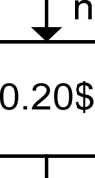
\includegraphics[width=1.26in,height=1.08in]{./image16} &

\includegraphics[width=0.747in,height=1.35in]{./image17} &
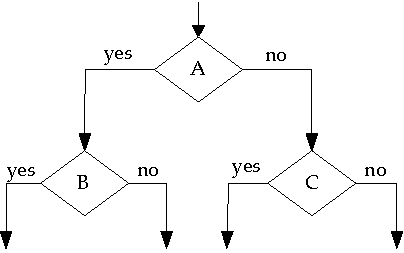
\includegraphics[width=2.16in,height=1.314in]{./image18} \\
(a) &  (b)  & (c) \\
\end{tabular}

\item
  Create a flowchart that outlines how to crochet a two-tone blanket
  with a diagonal stripe across it as shown below. A blanket is
  crocheted by linking together a sequence of basic stitches. For the
  purposes of the flowchart assume that a basic stitch is an elaborate
  process. Basic stitches are made from either dark or light yarn. The
  blanket should be 100 stitches wide by 150 stitches high. The diagonal
  stripe runs at a 45 degree angle from the horizontal.


\includegraphics[width=1in,height=1.34in]{./image19}


\item
  Build a data flow diagram and event table to represent an image
  archiving system for an art museum. The art museum maintains a
  database of digital images of paintings from museums all over the
  world. The following information is known about the image database
  system:

\begin{itemize}
\item
  Images are shared among museums in a participating network. Whenever a
  participating museum posts a new image, it sends a broadcast email to
  all participating museums in the network with the image attached as an
  email. It provides the name of the painting and artist in the body of
  the email. All new images received are added directly to the museum's
  own image database.
\item
  When inserted into the museum's database, each image is provided with
  a tag identifying the name of the painting and the artist.
  Furthermore, this triggers an image analysis routine that classifies
  the image based into predefined categories such as portrait, natural
  scene, and modern. Furthermore, it stores key features that are
  extracted from the image.
\item
  The key features are used to identify and retrieve visually similar
  images from the museum's database. Another image processing algorithm
  is run that compares the visual similarity of the new image to all
  images in the database. This process produces a matching score of 0 to
  100 that is stored.
\item
  The museum's image database is available to visitors via computer
  kiosks placed throughout the museum. Kiosk users can retrieve and view
  images in one of three ways. First, they can specify the name of the
  artist or painting. Second, they can retrieve a class of images, such
  as modern. Third, once they have received a painting, they can submit
  a request to view visually similar images. The visually similar images
  are retrieved for viewing based upon the matching score.
\end{itemize}

  \item
    Build an ERD to keep track of the bicycle frames manufactured at a
    local company. The following are notes from an interview with the
    owner.


\begin{quote}
\emph{We custom build bike frames to the dimension of each individual
customer. When a customer comes in we take measurements in their height,
leg length, arm length, torso length, weight, and waist measurement.
Since we have high customer satisfaction our customers order new frames
every several year. Hence we would like to date these measurements in
order to track how a customer's body changes through time .Each frame is
built on one set of measurements. Clearly, we need to keep track of our
customer's contact information like name, address, phone number, and
email address. We would like to know which employee built which frame.
We would like to store basic information like name, address, phone, and
SSN for each employee. Each frame is built by one employee using a
variety of different titanium tubing. We have strict inventory control
on all of our tubing and need to keep track of its grade, lot \#, Outer
Diameter (OD), Inner Diameter (ID), and manufacturer. Tubing is uniquely
identified by its lot \#. Finally we need to keep information on the
frame. Each frame is given a unique serial number, and has a color,
type, and dimensions.}
\end{quote}


\item
  Extend Problem~\ref{problem:stateDiagramTapeCartridges}
  to create an ERD that captures data about the tape
  cartridges used in the backup system. Every Sunday night a full backup
  is made of all network drives. A full backup creates an identical copy
  of the network drives on the tape cartridges. Due to the large amount
  of information, a full backup requires many tapes. On the other nights
  of the week an incremental backup is made. An incremental backup
  stores only files modified since the last backup (either full or
  incremental). Incremental backups are much smaller than a full backup,
  and consequently many incremental backups fit on a single tape. A tape
  contains only full or incremental backup information -- the unused
  portion of the last tape used for a full backup is never used to store
  incremental backups. Your company wants to keep track of tapes, full
  backups, and incremental backups. An ID and state should be tracked
  for each tape. For full backups, the system needs to track the
  creation date and the number of tapes used. For an incremental backup
  it should track the date it was made. The relationships between the
  backup type and the tape will capture which tapes participated in
  which backup. (Hint: the state of a tape should be an attribute of the
  tape entity - unformatted, blank, etc. They are not attributes and are
  possible values for the state attribute.)

\item
  \textbf{Project Application.} Develop behavior models that are
  applicable for describing your system. 
  Table~\ref{table:guidanceModelSelection} is provided to help
  in making the determination as to which models are applicable
\end{enumerate}

\section{Problems}
\label{section:testingProblems}

\begin{enumerate}
\def\labelenumi{\arabic{enumi}.}
\item
  Explain the differences between black box and white box testing.
\item
  Identify a circuit simulator (analog or digital) that you are familiar
  with. Explain the features of this simulator, which increase the
  observability and controllability of the circuit being simulated.
\item
  A mobile robot is being built. It uses a two DC motors in a
  differential drive configuration, a microcontroller to control
  movement and an ultrasonic sensor to detect obstacles. The robot is
  built to wander around without bumping into objects. Explain how stubs
  could be used in testing to take the place of incomplete subsystems.
  Be specific.
\item
  Consider that you have an op amp integrated circuit package, such as
  the LM741 in Appendix C. What type of testing would be appropriate for
  testing this device? Write a short test plan for doing so.
\item
  Explain under what situations a matrix test is appropriate.
\item
  Explain under what situations a step-by-step is test appropriate.
\item
  Consider the stages of unit testing, integration testing, and
  acceptance testing. For each of these stages, identify the
  corresponding requirements that each test should be traceable to.
\item
  Consider the case study robot design in Section~\ref{section:case-study-security-robot-design}, 
  which presents an
  acceptance test for the first system requirement. Develop an
  acceptance test for the second system requirement.
\item
  Consider the case study robot design in Section~\ref{section:case-study-security-robot-design}. 
  Develop an
  integration test that demonstrates the combined operation of the DC
  motors, MCU, and range finder.
\item
  Consider the case study robot design in Section~\ref{section:case-study-security-robot-design}. 
  Develop an
  integration test that demonstrates the combined operation of the
  digital compass, MCU, and LCD.
\item
  Consider the case study robot design in Section~\ref{section:case-study-security-robot-design}. 
  Develop unit
  tests for range finder, the DC motors, the H-bridges, and the LCD.
\item
  \textbf{Project Application.} Develop an acceptance test suite for
  your project. The acceptance tests should apply to the engineering
  requirements developed for the system.
\item
  \textbf{Project Application.} Develop an integration test suite for
  your project. The integration tests should apply to the higher levels
  of the design architecture and address the interaction between
  functional units.
\item
  \textbf{Project Application.} Develop a unit test quite for your
  project. The unit tests should apply to the lowest level units in the
  design.
\end{enumerate}

\section{Problems}
\label{section:problems}

\begin{enumerate}
\def\labelenumi{\arabic{enumi}.}
\item
  Consider a random variable that obeys a uniform density and varies
  from 2 to 5. (a) Determine the mean and variance of the random
  variable. (b) What is the probability that the random variable is
  between 2 and 3? (c) Plot the CDF.
\item
  In Figure 8.7 it was assumed that the CDF function is monotonically
  increasing. That is, \includegraphics{Fig/media/image162.wmf}. Show
  why this is so using equation (13).
\item
  Describe what is meant by \emph{failure rate}, \emph{failure
  function}, and \emph{reliability}.
\item
  Consider an integrated circuit that has
  \includegraphics{Fig/media/image163.wmf}. (a) Determine the mean time
  to failure. (b) Determine the reliability in 5, 10, 15, and 20 years.
\item
  Consider a CD4001BC 2-Input Quad NOR gate (datasheet available in
  Appendix D). Also assume it is a glass-sealed dual inline package, 15
  years in production, \includegraphics{Fig/media/image164.wmf}, the
  power dissipated in the application averages 10mW, it has B-1 quality,
  and that it is to be operated in laboratory equipment at an ambient
  temperature of 25°C. Use the MIL-HDBK-217F data in Appendix C to
  determine the MTTF and estimate its reliability in 25 years.
\item
  Use the MIL-HDBK-217F data in Appendix C to estimate the reliability
  of a 32 bit CMOS microprocessor. Assume that it is used in a missile
  launcher, the ambient temperature is 120°C, that it has 64 pins, that
  it has been in production for 6 months, B-1 quality parts are used,
  and it is a non-hermetic DIP. Determine the MTTF and reliability for
  the microprocessor in 20 years. (Note: this is the same operating
  environment used for the BJT in Example 8.5.)
\item
  Consider a 1N4001 diode (datasheet in Appendix D) that is to be
  operated in the switching circuit shown below. Also assume that the
  part quality is Lower, it is metallurgically bonded, and that it is to
  be used in an airborne inhabited cargo environment at an ambient
  temperature of 50°C. Use the MIL-HDBK-217F data in Appendix C to
  determine the MTTF and estimate its reliability in 25 years.
\end{enumerate}

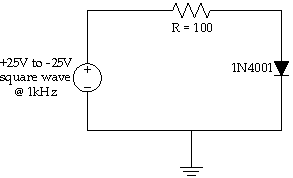
\includegraphics[width=2.5in,height=1.51042in]{Fig/media/image165.emf}

\begin{enumerate}
\def\labelenumi{\arabic{enumi}.}
\setcounter{enumi}{7}
\item
  Use the MIL-HDBK-217F data in Appendix C to determine the reliability
  of the inverting op amp circuit, shown below, in 15 years. Assume that
  it is used in an automotive application (environmental factor =
  G\textsubscript{M}), the ambient operating temperature is
  80\textsuperscript{O}C, industrial quality parts are employed, and ¼
  watt fixed composition resistors of the lowest quality are used. The
  datasheet for the LM741 op amp is in Appendix D. The LM741 is
  considered to be a linear microcircuit, comes in a dual inline package
  (DIP), contains 25 bipolar transistors, has S quality, and has been in
  production for well over 20 years.
\end{enumerate}

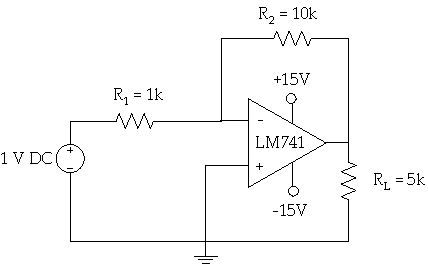
\includegraphics[width=2.8125in,height=1.77083in]{Fig/media/image166.emf}

\begin{enumerate}
\def\labelenumi{\arabic{enumi}.}
\setcounter{enumi}{8}
\item
  Consider the circuit in Example 8.4. Assume that a heat sink is
  attached to the 2N3904 BJT (datasheet in Appendix D) and it has the
  following thermal resistance values
  \includegraphics{Fig/media/image167.wmf} and
  \includegraphics{Fig/media/image168.wmf}. If the device is operated at
  an ambient temperature of 130°C, determine the maximum power
  dissipation of the BJT and its reliability in 50 years.
\item
  Your company intends to design, manufacture, and market a new RAID
  (Redundant Array of Independent Disks) for network servers. The system
  must be able to store a total of 500GB of user data and must have a
  reliability of at least 95\% in 10 years. In order to develop the RAID
  system, 20GB drives will be designed and utilized. To meet the
  requirement, you have decided to use a bank of 25 disks
  (25x20GB=500GB) and utilize a system redundancy of 4 (each of the 25
  disks has a redundancy of 4). What must the reliability of the 20GB
  drive be in 10 years in order to meet the overall system reliability
  requirement?
\item
  \includegraphics{Fig/media/image106.wmf} has a failure probability of
  2\% and \includegraphics{Fig/media/image169.wmf} has a failure
  probability of 3\%. \includegraphics{Fig/media/image170.wmf},
  \includegraphics{Fig/media/image171.wmf},
  \includegraphics{Fig/media/image172.wmf}, and
  \includegraphics{Fig/media/image173.wmf} are identical redundant
  systems. Determine the required reliability of the redundant systems
  necessary for the overall system to have a reliability of 94\%.
\end{enumerate}

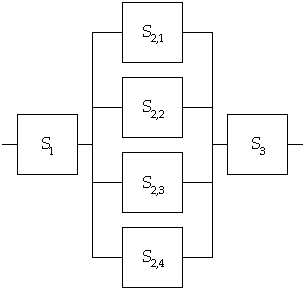
\includegraphics[width=2.0625in,height=1.96875in]{Fig/media/image174.emf}

\begin{enumerate}
\def\labelenumi{\arabic{enumi}.}
\setcounter{enumi}{11}
\item
  Consider the design of a triply-redundant majority voting system, with
  three binary inputs a, b, and c shown below. The inputs represent data
  from 3 independent sources from which the objective is to determine if
  the majority of the input bit values are logic level 0 or 1. Each
  majority circuit outputs the bit value that is in the majority of the
  inputs. The output of each majority circuit is fed into a resistor and
  LED (light emitting diode) network. The LEDs are lit if the output of
  the majority circuit is a logic 1, otherwise the LED is off. Ideally,
  all three LEDs are lit if the majority of inputs is 1, else they are
  all off. However, if part of the system fails, the LED readings may
  not be reliable, so a majority rules decision is used on the LEDs. The
  criterion used is that if two or more LEDs are on, then the majority
  of inputs are considered to be high, otherwise, the majority of inputs
  are considered to be low. Determine the probability of a false reading
  based upon this criterion if each component in the system (gate,
  resistor, or LED) has a reliability of 90\%.
\end{enumerate}

\begin{quote}
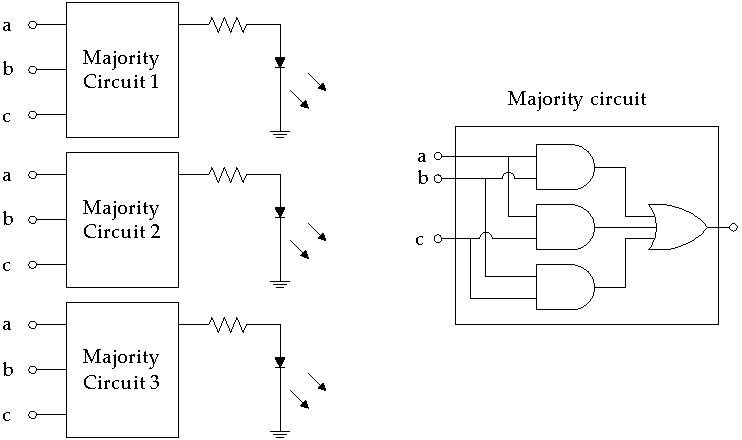
\includegraphics[width=4.1875in,height=2.48958in]{Fig/media/image175.emf}
\end{quote}

\section{Problems}
\label{section:teamsProblems}

\begin{enumerate}
\def\labelenumi{\arabic{enumi}.}
\item
  Explain the difference between cross-functional and multi-disciplinary
  teams.
\item
  Identify the characteristics of the forming, storming, norming and
  performing stages in team development.
\item
  Describe the distinction between teams and teamwork.
\item
  According to this chapter, it is difficult to develop a consensus as
  the number of team members increases. Consider the situation where a
  team needs to agree on a proposal. Furthermore, assume that each team
  member's vote is random with a 50\% chance of agreeing with the
  proposal. Plot the probability of the team unanimously agreeing to the
  proposal versus the number of team members. Consider team sizes from 2
  to 10. Overlay three additional plots for the situation where each
  team member has a 75\%, 90\%, and 99\% chance of agreeing to the
  proposal.
\item
  \textbf{Project Application.} Develop Team Process Guidelines as
  proposed in 
Section~\ref{section:project-application-team-process-guidelines}
\item
  \textbf{Project Application}. Complete the team self-assessment in
  Table~\ref{table:teamCheckList}.
\end{enumerate}

\subsection{Problems}\label{problems}

\begin{enumerate}
\def\labelenumi{\arabic{enumi}.}
\item
  In your own words, describe what is meant by the work breakdown
  structure.
\item
  Consider the set of activities, duration (in days), and predecessors
  for a project given below.
\end{enumerate}

\begin{longtable}[]{@{}
  >{\raggedright\arraybackslash}p{(\columnwidth - 18\tabcolsep) * \real{0.1354}}
  >{\raggedright\arraybackslash}p{(\columnwidth - 18\tabcolsep) * \real{0.0961}}
  >{\raggedright\arraybackslash}p{(\columnwidth - 18\tabcolsep) * \real{0.0961}}
  >{\raggedright\arraybackslash}p{(\columnwidth - 18\tabcolsep) * \real{0.0961}}
  >{\raggedright\arraybackslash}p{(\columnwidth - 18\tabcolsep) * \real{0.0961}}
  >{\raggedright\arraybackslash}p{(\columnwidth - 18\tabcolsep) * \real{0.0961}}
  >{\raggedright\arraybackslash}p{(\columnwidth - 18\tabcolsep) * \real{0.0961}}
  >{\raggedright\arraybackslash}p{(\columnwidth - 18\tabcolsep) * \real{0.0961}}
  >{\raggedright\arraybackslash}p{(\columnwidth - 18\tabcolsep) * \real{0.0961}}
  >{\raggedright\arraybackslash}p{(\columnwidth - 18\tabcolsep) * \real{0.0961}}@{}}
\toprule\noalign{}
\begin{minipage}[b]{\linewidth}\raggedright
\textbf{Activity}
\end{minipage} & \begin{minipage}[b]{\linewidth}\raggedright
A
\end{minipage} & \begin{minipage}[b]{\linewidth}\raggedright
B
\end{minipage} & \begin{minipage}[b]{\linewidth}\raggedright
C
\end{minipage} & \begin{minipage}[b]{\linewidth}\raggedright
D
\end{minipage} & \begin{minipage}[b]{\linewidth}\raggedright
E
\end{minipage} & \begin{minipage}[b]{\linewidth}\raggedright
F
\end{minipage} & \begin{minipage}[b]{\linewidth}\raggedright
G
\end{minipage} & \begin{minipage}[b]{\linewidth}\raggedright
H
\end{minipage} & \begin{minipage}[b]{\linewidth}\raggedright
I
\end{minipage} \\
\midrule\noalign{}
\endhead
\bottomrule\noalign{}
\endlastfoot
\textbf{Duration} & 3 & 9 & 6 & 6 & 6 & 3 & 2 & 6 & 7 \\
\textbf{Predecessors} & - & - & - & A,B & D,B & C & F,E & G & F \\
\end{longtable}

\begin{enumerate}
\def\labelenumi{\alph{enumi})}
\item
  Develop a network diagram representation for the project.
\item
  Determine the critical path.
\item
  Determine the float time for all activities that are not on the
  critical path.

  \begin{enumerate}
  \def\labelenumii{\arabic{enumii}.}
  \item
    Consider the set of activities, duration (in days), and predecessors
    for a project given below.
  \end{enumerate}
\end{enumerate}

\begin{longtable}[]{@{}
  >{\raggedright\arraybackslash}p{(\columnwidth - 22\tabcolsep) * \real{0.1644}}
  >{\raggedright\arraybackslash}p{(\columnwidth - 22\tabcolsep) * \real{0.0758}}
  >{\raggedright\arraybackslash}p{(\columnwidth - 22\tabcolsep) * \real{0.0761}}
  >{\raggedright\arraybackslash}p{(\columnwidth - 22\tabcolsep) * \real{0.0757}}
  >{\raggedright\arraybackslash}p{(\columnwidth - 22\tabcolsep) * \real{0.0769}}
  >{\raggedright\arraybackslash}p{(\columnwidth - 22\tabcolsep) * \real{0.0755}}
  >{\raggedright\arraybackslash}p{(\columnwidth - 22\tabcolsep) * \real{0.0754}}
  >{\raggedright\arraybackslash}p{(\columnwidth - 22\tabcolsep) * \real{0.0757}}
  >{\raggedright\arraybackslash}p{(\columnwidth - 22\tabcolsep) * \real{0.0769}}
  >{\raggedright\arraybackslash}p{(\columnwidth - 22\tabcolsep) * \real{0.0757}}
  >{\raggedright\arraybackslash}p{(\columnwidth - 22\tabcolsep) * \real{0.0766}}
  >{\raggedright\arraybackslash}p{(\columnwidth - 22\tabcolsep) * \real{0.0755}}@{}}
\toprule\noalign{}
\begin{minipage}[b]{\linewidth}\raggedright
\textbf{Activity}
\end{minipage} & \begin{minipage}[b]{\linewidth}\raggedright
A
\end{minipage} & \begin{minipage}[b]{\linewidth}\raggedright
B
\end{minipage} & \begin{minipage}[b]{\linewidth}\raggedright
C
\end{minipage} & \begin{minipage}[b]{\linewidth}\raggedright
D
\end{minipage} & \begin{minipage}[b]{\linewidth}\raggedright
E
\end{minipage} & \begin{minipage}[b]{\linewidth}\raggedright
F
\end{minipage} & \begin{minipage}[b]{\linewidth}\raggedright
G
\end{minipage} & \begin{minipage}[b]{\linewidth}\raggedright
H
\end{minipage} & \begin{minipage}[b]{\linewidth}\raggedright
I
\end{minipage} & \begin{minipage}[b]{\linewidth}\raggedright
J
\end{minipage} & \begin{minipage}[b]{\linewidth}\raggedright
K
\end{minipage} \\
\midrule\noalign{}
\endhead
\bottomrule\noalign{}
\endlastfoot
\textbf{Duration} & 9 & 12 & 3 & 4 & 5 & 9 & 8 & 3 & 6 & 9 & 1 \\
\textbf{Predecessors} & - & A & A & B,C & C & B & D & F,D & G & H,I &
E \\
\end{longtable}

\begin{enumerate}
\def\labelenumi{\alph{enumi})}
\item
  Develop a network diagram representation for the project.
\item
  Determine the critical path.
\item
  Determine the float time for all activities that are not on the
  critical path.

  \begin{enumerate}
  \def\labelenumii{\arabic{enumii}.}
  \item
    Explain why a network diagram cannot contain cycles. A cycle is a
    sequence of activities where you can travel back to an activity
    already visited.
  \item
    Describe the advantages and disadvantages of the network diagram and
    Gantt chart representations for a project.
  \item
    Assume that the following data has been determined for the
    development and sale of a new digital thermometer for home use:
    development cost = \$250,000, production investment = \$500,000,
    annual production volume = 20,000 units per year, and the sales
    lifetime is 7 years. Assuming a variable production cost of \$5 per
    unit, determine: (a) the sales price necessary to break even within
    2 years, and (b) the profit expected over the estimated sales
    lifetime.
  \item
    Describe the difference between the cost estimation models in
    equations (7) and (8) and the COCOMO cost estimation model.
  \item
    Consider a software development project that has a team of 50
    software development engineers. The team has proposed a design and
    estimates that it will require 500,000 lines of code to complete the
    project. The average cost to the company for an engineer is \$90,000
    per year, including salary, benefits, and overhead. Estimate (a) the
    time required to complete the project, and (b) the labor costs.
  \item
    Consider a software development project where the team has proposed
    a design and estimates that it will require 200,000 lines of code to
    complete. The average cost to the company for an engineer is
    \$110,000 per year, including salary, benefits, and overhead.
    Estimate (a) the number of engineers needed to complete the project
    within 18 months, and (b) the labor costs.
  \item
    \textbf{Project Application.} Develop a project plan for your
    project. A format and guideline for developing the plan is contained
    in Section 10.7.
  \end{enumerate}
\end{enumerate}

\chapter{Problems}


\begin{enumerate}
\def\labelenumi{\arabic{enumi}.}
\item
  Describe the relationship between ethics and morals.
\item
  Describe the differences between morals and values.
\item
  Which patent is most relevant for engineering inventions, a design
  patent or utility patent? Why?
\item
  What are the criteria that are used in evaluating patents?
\item
  Explain the importance of claims in a patent application.
\item
  Discuss the tradeoffs involved between using patents and trade secrets
  to protect intellectual property.
\item
  When can reverse-engineering be used, and how can the information
  obtained from it be used?
\item
  What is the difference between negligence and strict liability in tort
  law?
\item
  For the case study presented below, apply the ethical decision making
  paradigm presented in Section 11.5 to analyze the situation. Present
  potential solutions to the scenario and provide a discussion of them.

\begin{quote}
\ul{\hfill\break
Case Study: Disk Drive Diagnostics. (Copyright John Wallberg. Reprinted
by permission.)}

SCSI, an industry standard system for connecting devices (like disks) to
computers, provides a vendor ID protocol by which the computer can
identify the supplier (and model) of every attached disk.

Company C makes file servers consisting of a processor and disks. Disks
sold by C identify C in their vendor ID. Disks from other manufacturers
can be connected to C\textquotesingle s file servers; however, the file
server software performs certain maintenance functions, notably
pre-failure warnings based on performance monitoring, only on C-supplied
disks.

Company P decides to compete with C by supplying cheaper disks for
C\textquotesingle s file server. They quickly discover that while their
disks work on C\textquotesingle s file servers, their disks lack a
pre-failure warning feature that C\textquotesingle s disks have.
Therefore, the CEO of P directs you, the engineer in charge of the disk
product, to find a solution to the problem of no pre-failure warning for
your disks. Using reverse engineering, you discover that by changing the
vendor ID of P's disks, the C file servers will treat P disks as C
disks. Your management at company P instructs you to incorporate this
change into your product so that you can advertise the disks as ``100\%
C-compatible.'' What would you do in this situation?
\end{quote}


\item
  For the case study presented below, apply the ethical decision making
  paradigm presented in Section 11.5 to analyze the situation. Present
  potential courses of action and provide a discussion of them.


\begin{quote}
\ul{Case Study: Encryption Software} (Texas A\&M Ethics Case Studies,
\url{http://ethics.tamu.edu}. Reprinted by permission.)

You are a recently hired engineer who has been recruited directly out of
college. For your first assignment, your boss asked you to write a piece
of software to provide security from "prying eyes" over e­mailed
documents; these documents would be used internally by the company. This
software will subsequently be distributed to different departments.

Upon completion of this software project, you saw a program on the local
news about an individual in California who has made similar software
available overseas. This individual is currently under prosecution in a
federal court for the distribution of algorithms and information which
(by law) must remain within the United States for purposes of national
security.

It occurs to you that your company is a multinational corporation and
that the software might have been distributed overseas. You then
discover that the software has indeed been sent overseas to other
offices within the corporation. You speak with your boss, informing him
of the news program from the night before. He shrugs off this comment,
stating that ``The company is based in the United States and we are
certainly no threat to national security in any way. Besides,
there\textquotesingle s no way anyone will find out about software we
use internally.''

You agree with your boss, and let it go. Later on however, you receive a
letter from a gentleman working as a contractor for his company
overseas. Through some correspondence regarding the functionality of the
software and technical matters, you learn that the Middle Eastern office
had been supplying his software outside the company to contractors and
clients so that they could exchange secure e­mailed documents. What would
you do in this situation?
\end{quote}


\item
  For the case study presented below, apply the ethical decision making
  paradigm presented in Section 11.5 to analyze the situation. Present
  potential courses of action and provide a discussion of them.

\begin{quote}
\ul{Case Study: A Failure.} (Texas A\&M Ethics Case Studies,
\url{http://ethics.tamu.edu}. Reprinted by permission.)

You work for Velky Measurement which has for years provided DGC
Corporation with sophisticated electronic equipment for patient health
monitoring systems. Recently, DGC returned a failed piece of measurement
equipment. A meeting was held with representatives of Velky and DGC to
discuss the problem. This included you and your project manager who is
intimately acquainted with the returned equipment. During the course of
the meeting it becomes apparent to you that the problem has to be
Velky\textquotesingle s. You suspect that the equipment failed because
of an internal design problem and that it was not properly tested.
However, at the conclusion of the meeting your project manager
represents Velky's official position---the test equipment is functioning
properly.

You keep silent during the meeting, but afterwards talk to your project
manager about his diagnosis. You suggest that Velky tell DGC that the
problem is due to a design fault and that Velky will replace the
defective equipment. You manager replies, ``\emph{I
don\textquotesingle t think it\textquotesingle s wise to acknowledge
that it\textquotesingle s our fault. There\textquotesingle s no need to
hang out our wash and lessen DGC\textquotesingle s confidence in the
quality of our work. A good will gesture to replace the equipment should
suffice}.''

Utlimately, Velky's management replaces the equipment because DGC has
been such a good customer. Although Velky replaces the equipment at its
own expense, it does not disclose the real nature of the problem. What
would you do in this situation?
\end{quote}

\item
  For the case study presented below, apply the ethical decision making
  paradigm presented in Section 11.5 to analyze the situation. Present
  potential courses of action and provide a discussion of them.

\begin{quote}
\ul{Case Study: A Vacation} (Texas A\&M Ethics Case Studies,
\url{http://ethics.tamu.edu}. Reprinted by permission.)

You work for Rancott and were looking forward to an upcoming trip for
weeks. Once you were assigned to help install Rancott's equipment for
Boulding Corporation, you arranged a vacation at a nearby ski resort.
The installation was scheduled to be completed on the
12\textsuperscript{th} and your vacation would begin on the
13\textsuperscript{th}. That meant a full week of skiing with three of
your old college buddies.

Unfortunately, not all of the equipment arrived on time. Eight of the
ten identical units were installed by mid-morning on the
12\textsuperscript{th}. Even if the remaining two units had arrived that
morning, it would take another full day to install them. However, you
were informed that it might take as long as two more days for the units
to arrive.

``\emph{Terrific,}'' you sighed, ``\emph{there goes my vacation---and
all the money I put down for the condo}.'' ``\emph{No problem},''
replied Jerry, the Boulding engineer who had worked side-by-side with
you as each of the first eight units was installed. He said ``\emph{I
can handle this for you. We did the first eight together.
It\textquotesingle s silly for you to have to hang around and blow your
vacation}.'' Jerry knew why you were sent to supervise the installation
of the new equipment. It had to be properly installed in order to avoid
risking injuries to those who use it. Although you are aware of this,
you are confident that Jerry is fully capable to supervise the
installation of the remaining two units. What would you do?
\end{quote}

\end{enumerate}
\include{./chapter12/problemSet12}
\end{comment}

\end{document} 
